%!TEX root = ../iotpaper.tex

%~~~~~~~~~~~~~~~~~~~~~~~~~~~~~~~~~~~~~~~~~~~~~~~~~~~~~~~~~~~~~~~


\section{Gesture Library Experiments}
\label{sec:GestureLibrary}

\begin{table}

\begin{center}
  \begin{tabular}{ c | c | c | c  }
    \hline
    1 & 2 & 3 & 4  \\ \hline
    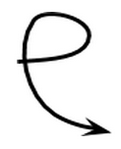
\includegraphics[width=0.2\linewidth, height=13mm]{./figures/gesture_e.png} & 
    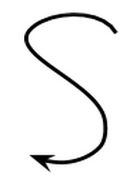
\includegraphics[width=0.2\linewidth, height=13mm]{./figures/gesture_s.png} &
    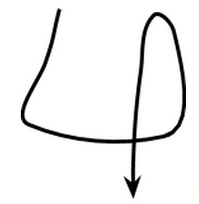
\includegraphics[width=0.2\linewidth, height=13mm]{./figures/gesture_num4.png} &
    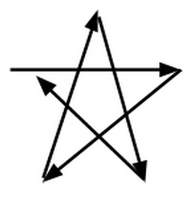
\includegraphics[width=0.2\linewidth, height=13mm]{./figures/gesture_star.png}  \\ \hline
    5 & 6 & 7 & 8 	 \\ \hline
    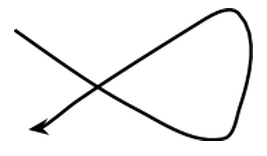
\includegraphics[width=0.2\linewidth, height=13mm]{./figures/gesture_5.png} &
    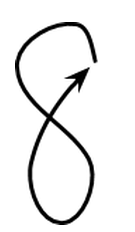
\includegraphics[width=0.2\linewidth, height=13mm]{./figures/gesture_num8.png} &
    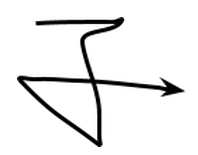
\includegraphics[width=0.2\linewidth, height=13mm]{./figures/gesture_7.png} &
    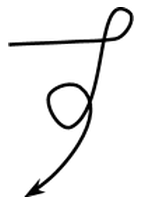
\includegraphics[width=0.2\linewidth, height=13mm]{./figures/gesture_su.png}  \\ \hline
    9 & 10 & 11 & 12  \\ \hline
    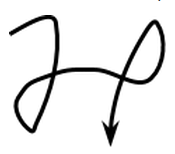
\includegraphics[width=0.2\linewidth, height=13mm]{./figures/gesture_mi.png} & 
    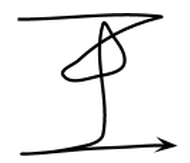
\includegraphics[width=0.2\linewidth, height=13mm]{./figures/gesture_wang.png} &
    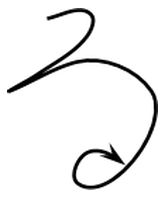
\includegraphics[width=0.2\linewidth, height=13mm]{./figures/gesture_ru.png} &
    
\includegraphics[width=0.2\linewidth, height=13mm]{./figures/gesture_miu.png}	\\ \hline
    13 & 14 & 15 & 16  \\ \hline
    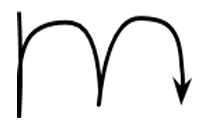
\includegraphics[width=0.2\linewidth, height=13mm]{./figures/gesture_m.png} &
    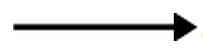
\includegraphics[width=0.2\linewidth, height=13mm]{./figures/gesture_14.png} &
    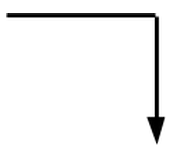
\includegraphics[width=0.2\linewidth, height=13mm]{./figures/gesture_15.png} & 
    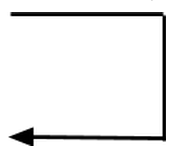
\includegraphics[width=0.2\linewidth, height=13mm]{./figures/gesture_16.png}  \\ \hline
    17    \\ \hline
    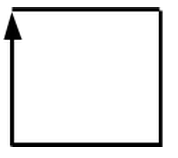
\includegraphics[width=0.2\linewidth, height=13mm]{./figures/gesture_17.png} \\ \hline
  \end{tabular}
\end{center}
\caption{Gestures for authentication} % title of Table
\label{table:GestureTable}
\end{table}


To test the Gesture Library Model, we collect gesture data from all three group members. Our experimental library consists of the 17 different gestures shown in \autoref{tab:GestureTable}. These gestures are a mix of European characters, Asian characters, and simple shapes, each with varying complexity. 

Gino is the legitimate user who performed calibration on his iPhone 6 device. To emulate a strong attacker, Henry attempts authentication using a second iPhone 6 device. Joe is a weaker attacker who attempts authentication on an iPhone 6s. Joe is less familiar with Asian characters, and thus is weaker than Henry because of the selecting gestures. Gino also attempts authentication on his second device, the Nexus 5, as a legitimate user.

For each gesture, Gino takes 30 calibration attempts on his iPhone 6. Afterwards, everyone attempts 10 new authentications for each gesture each day. In the next sections, we discuss calibration and set thresholds that minimize false negatives (rejecting Gino, the legitimate user), while also minimizing false positives (accepting Henry or Joe, the attackers).

\subsection{Calibration Mechanism}

Our calibration mechanism is a brute force search that calculates the \gls{DTW} distance of one attempt time series to another for the same gesture. The calibrated time series selected is the attempt with the smallest average distance to all of the other attempts. This approach is non-scalable ($O(N^{2})$ where $N$ is the number of calibration attempts). However, scalability is not the focus of this project because we can make calibration a one-time event at the beginning and choose not to update the history for the purposes of this experiment. For calibration, we use the full 30 attempts per gesture data set unless otherwise noted.

\subsection{Gesture Distance Consistency}

First, to prove that gesture-based authentication works, we monitor the consistency of the \gls{DTW} from the calibration time series over the period of 7 days for both the legitimate user and the attackers. We hypothesize that the average distance for all the attempts for a single gesture on a single day from the attackers stays at least one standard deviation away from the average distance for the intended user. Furthermore, we hypothesize that the intended user's average distance should stay within one standard deviation of the previous day's average.

\hl{DATA HERE}

\subsection{Threshold Setting}

\subsubsection{Technique}

The threshold for rejecting or accepting a user can be set using a variety of techniques. For this project, we use a simple threshold ($D_{t}$) based on the calibration data above as a proof of concept. Each attempt from calibration has an average \gls{DTW} distance from all of the other calibration attempts. Based on this distance, we can set a threshold tailored to gesture $i$ using \autoref{eq:thres}

\begin{equation}
D_{t} = m \cdot d_{i} + \frac{1.96 \cdot \delta_{i}}  {\sqrt{N}}
\label{eq:thres}
\end{equation}

\noindent where $m$ is a constant multiplicative factor, $d_{i}$ is a mean distance value based on the distance data from calibration for gesture $i$, and $\delta_{i}$ is the associated standard deviation.

Intuition suggests that choosing the minimum recorded \gls{DTW} distance for $d_{i}$ yields an overly strict system that minimizes false positives but also introduces additional false negatives to the system. Likewise, choosing the maximum recorded \gls{DTW} distance for $d_{i}$ produces an overly lenient system that minimizes false positives but introduces false negatives. 

To make the system more usable, we opt to split the difference to minimize both false positives and false negatives. However, if we must choose between more false positives and false negatives, we choose to err on the side of more false positives to make the system more usable to the end user. Therefore, we set $d_{i}$ based on the 80th, 85th, and 90th percentiles of the calibration data. This lets us minimize the effects of any major calibration outliers while still being lenient. Furthermore, the multiplicative factor $m$ is used to introduce some additional leniency because of day-to-day variation in the intended user's gesture. $m$ is varied from 1 to 5 in steps of 0.25.

Our hypothesis is that we can set an authentication distance threshold that keeps the false positives and false negatives rates averaged over all gestures below 10\% for all gestures.

\subsubsection{Results}

The optimal threshold settings are the ones that minimize both the false positives and false negatives. \autoref{fig:ThresFig} shows the results for false positives and false negatives for the (a) 80th, (b) 85th, and (c) 90th percentiles. For readability, we only include. $m$ values of 2, 2.5, and 3 in this figure.

\hl{Talk about the plots here}.

\subsection{Number of Calibration Iterations}

Thus far, our evaluation is based on our full data set of 30 calibration attempts per gesture. In this section, we investigate the performance of our Gesture Library model for smaller subsets of calibration attempts: 5, 15, and 30. We hypothesize that we will have more false positives and false negatives for the same parameters because of the smaller data set.

\hl{DATA HERE}.

\subsection{Multi-Attempt Authentication}

Placeholder

%~~~~~~~~~~~~~~~~~~~~~~~~~~~~~~~~~~~~~~~~~~~~~~~~~~~~~~~~~~~~~~~
 

